%%%%%%%%%%%%%%%%%%%%%%%%%%%%%%%%%%%%%%%%%%%%%%%%%%%%%%%%%%%%%%%%%%%%%%%%%%%%%%%%
%% 
\cleardoubleoddpage%  Make sure to start each chapter on a new odd page
\chapter{Background and Related Work}
\label{sec:background}


\section{Biosignal Processing and BIOT Architecture}
\label{sec:background:biot}

Biosignal processing is a central challenge in biomedical engineering. The main task is to analyze multi-channel time series data and extract clinically relevant information. Traditional approaches relied on handcrafted features and domain-specific preprocessing techniques. With the development of deep learning, more advanced and automated approaches have become possible.

\subsection{Challenges in Biosignal Processing}

Biosignals, such as \ac{EEG} and \ac{ECG}, are multi-channel time series recorded at high sampling rates in various healthcare domains. Automated analysis of these signals faces multiple interconnected challenges.

\textbf{Domain Shift and Generalization:} Machine learning models trained on biosignal data from one clinical site frequently exhibit poor performance when applied to recordings from different institutions~\cite{yang2023biot}. This cross-dataset generalization problem stems from systematic differences in recording equipment, clinical protocols, and patient populations. \ac{BIOT} demonstrates that conventional deep learning approaches typically require extensive retraining when applied to new data sources~\cite{yang2023biot}.

\textbf{Recording Duration Variability:} Clinical practice produces biosignal recordings of widely varying lengths. Diagnostic \ac{EEG} sessions may span 20-60 minutes, while ambulatory monitoring can extend over multiple days. Traditional neural network architectures designed for fixed-size inputs struggle to accommodate this temporal variability without extensive padding or truncation, which can distort the underlying signal characteristics.

\textbf{Incomplete and Corrupted Data:} Real-world clinical recordings frequently contain missing channels due to electrode displacement, amplifier saturation, or deliberate protocol changes~\cite{banville2022robust}. Individual time segments may be corrupted by patient movement, environmental interference, or equipment malfunction. Conventional approaches require imputation or data exclusion, potentially introducing artifacts or reducing statistical power.

\textbf{Heterogeneous Format Specifications:} As emphasized in the \ac{BIOT} framework~\cite{yang2023biot}, biosignal datasets exhibit substantial format diversity. Seizure detection studies might employ 16-channel bipolar montages sampled at 256~Hz, while sleep staging research commonly uses different electrode configurations and sampling frequencies. Channel naming conventions, reference schemes, and signal scaling practices vary across recording systems, complicating cross-dataset model development.

\subsection{BIOT: Biosignal Transformer Architecture}

The \acf{BIOT} architecture was developed to address these challenges through a unified framework capable of handling heterogeneous biosignal formats~\cite{yang2023biot}. Drawing inspiration from the Vision Transformer (ViT)~\cite{dosovitskiy2021vit} and Audio Spectrogram Transformer (AST)~\cite{gong2021ast}, \ac{BIOT} adapts the concept of tokenization, originally developed for images and audio, to biosignal data.

\begin{figure}[t]
\centering
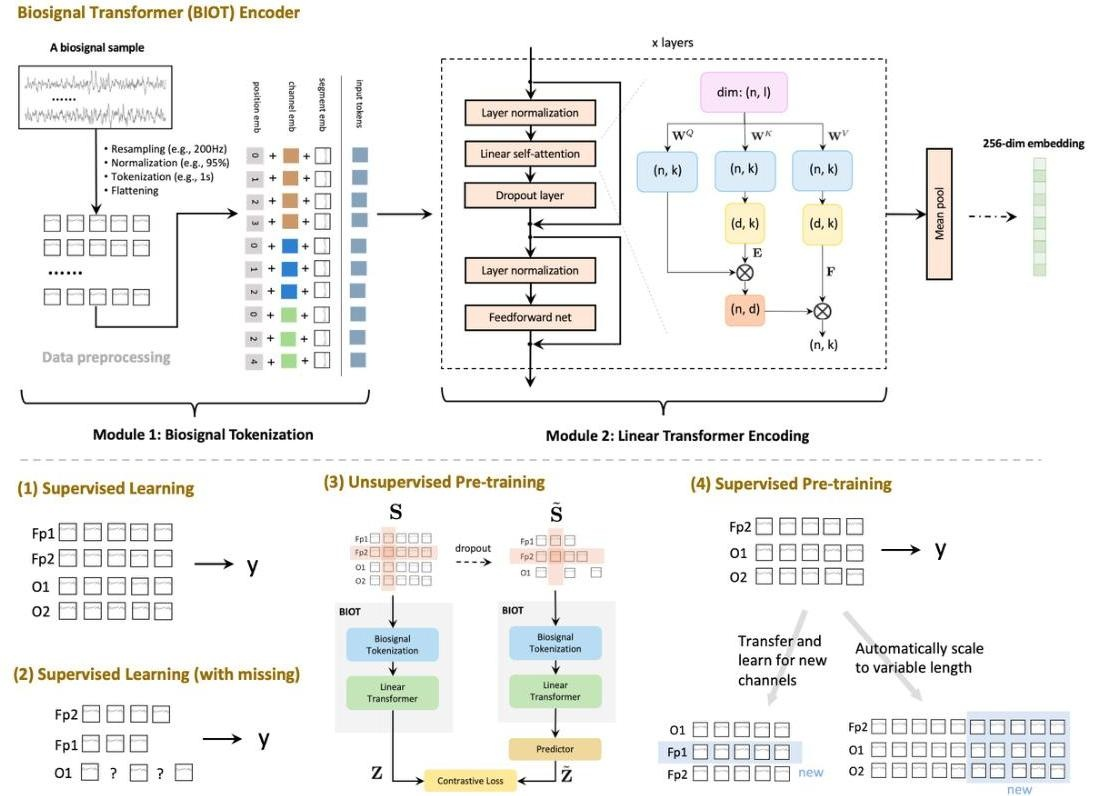
\includegraphics[width=0.95\linewidth]{images/biot_extracted_images/page_3_img-0.jpeg}
\caption{
    BIOT Architecture Overview (adapted from~\cite{yang2023biot}). Upper: Biosignal tokenization module transforms heterogeneous biosignals into unified "sentences", followed by linear transformer processing. Lower: BIOT's versatility across different learning scenarios including supervised learning, missing data handling, and pre-training approaches.
}\label{fig:biot_architecture}
\end{figure}

\subsubsection{Biosignal Tokenization Module}

A central design element of \ac{BIOT} is the concept of ``biosignal tokenization''~\cite{yang2023biot}. This approach transforms heterogeneous biosignals into unified ``sentence'' structures, enabling consistent processing across diverse recording formats:

\begin{figure}[t]
\centering
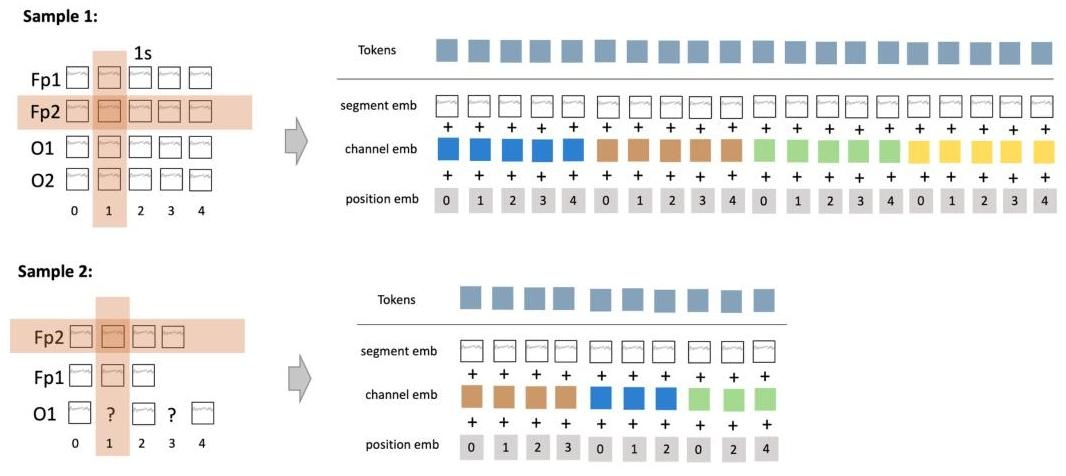
\includegraphics[width=0.95\linewidth]{images/biot_extracted_images/page_4_img-1.jpeg}
\caption{
    Biosignal Tokenization Process (adapted from~\cite{yang2023biot}). Sample 1 demonstrates standard tokenization with four channels (Fp1, Fp2, O1, O2) over 5 seconds. Sample 2 illustrates BIOT's flexibility with mismatched channels (missing O2), variable lengths, and missing values in O1. Different colors represent different channels, and the orange area shows spatial, temporal relationships between tokens.
}\label{fig:biot_tokenization}
\end{figure}

\paragraph{Resampling and Normalization}
Let $\mathbf{S} \in \mathbb{R}^{I \times J}$ denote a biosignal sample where $I$ denotes the number of channels and $J$ represents the temporal length in samples. The \ac{BIOT} preprocessing pipeline begins with resampling all channels to a standardized sampling rate~\cite{yang2023biot}. For \ac{EEG} applications, \ac{BIOT} employs 200~Hz, justified by the Nyquist-Shannon sampling theorem~\cite{Nyquist1928,Shannon1949} as sufficient for capturing frequencies up to 100~Hz, thereby covering clinically relevant \ac{EEG} bands~\cite{yang2023biot}.

Following resampling, \ac{BIOT} applies channel-wise normalization using the 95th percentile of absolute amplitude values~\cite{yang2023biot}:
$$\mathbf{S}_{norm}[i] = \frac{\mathbf{S}[i]}{\text{percentile}_{95}(|\mathbf{S}[i]|)}$$

This percentile-based strategy provides robustness against extreme amplitude artifacts while preserving relative amplitude relationships~\cite{yang2023biot}.

\paragraph{STFT-based Tokenization}
Rather than segmenting raw time-series data directly, the \ac{BIOT} framework applies the \acf{STFT} to transform temporal windows into frequency-domain representations~\cite{yang2023biot}. This spectral tokenization represents the core methodological innovation of \ac{BIOT}.

The tokenization proceeds as follows:

\textbf{Step 1 - Channel-wise Processing:} Each channel is processed independently. For channel $i$, the \ac{STFT} is applied with parameters:
\begin{itemize}
    \item \textbf{FFT Size ($N$):} Typically 200 samples (1 second at 200 Hz)
    \item \textbf{Hop Length ($H$):} Typically 100 samples (0.5 second stride)
    \item \textbf{Window Function:} Hann window for spectral smoothing
    \item \textbf{Centering:} Disabled (\texttt{center=False}) to maintain exact temporal alignment
\end{itemize}

\textbf{Step 2 - Frequency Spectrum Extraction:} The \ac{STFT} transforms each temporal window into a complex-valued frequency spectrum. Taking only the magnitude (absolute value) yields a real-valued representation:
$$\text{STFT}(\mathbf{S}[i]) \in \mathbb{R}^{F \times T}$$
where $F = N/2 + 1$ is the number of frequency bins (101 bins for $N=200$, spanning 0-100 Hz) and $T$ is the number of temporal frames.

\textbf{Step 3 - Token Count Calculation:} For a signal of length $J$ samples, the number of tokens generated per channel is:
$$T = \left\lfloor \frac{J - N}{H} \right\rfloor + 1$$

For example, a 5-second \ac{EEG} window (1000 samples at 200 Hz) produces:
$$T = \left\lfloor \frac{1000 - 200}{100} \right\rfloor + 1 = 9 \text{ tokens per channel}$$

With 16 channels, this yields $16 \times 9 = 144$ total tokens. This dramatic reduction from 1000 time-domain samples to 144 frequency-domain tokens makes the representation tractable for sequence models while preserving essential spectral information.

\textbf{Advantages of Channel-wise Processing:} Independent channel processing in \ac{BIOT} provides several advantages over approaches that segment all channels simultaneously~\cite{yang2023biot}:
\begin{itemize}
    \item \textbf{Missing Channel Robustness:} Absent channels can simply be omitted from the token sequence without requiring imputation or padding~\cite{yang2023biot}
    \item \textbf{Variable Length Handling:} Different channels can have different temporal extents without creating structural conflicts~\cite{yang2023biot}
    \item \textbf{Corrupted Segment Handling:} Individual tokens containing artifacts can be dropped without affecting neighboring channels~\cite{yang2023biot}
\end{itemize}

\paragraph{Token Embedding}
Each frequency-domain token must be transformed into a fixed-dimensional embedding suitable for sequence processing. \ac{BIOT} achieves this through three complementary embedding components that capture spectral content, spatial location, and temporal order (see Figure~\ref{fig:biot_tokenization}).

\textbf{1. Segment Embedding - Frequency Content Representation}

The \ac{STFT} output for each token is a frequency spectrum vector $\mathbf{f} \in \mathbb{R}^{F}$ where $F = N/2 + 1$ (e.g., 101 frequency bins for $N=200$). This vector represents the magnitude of each frequency component from 0 Hz to the Nyquist frequency (100 Hz at 200 Hz sampling rate).

The \texttt{PatchFrequencyEmbedding} module projects the frequency vector $\mathbf{f}$ into a higher-dimensional embedding $\mathbf{e}_{segment} \in \mathbb{R}^{d}$ through a learned linear transformation:
$$\mathbf{e}_{segment} = \mathbf{W}_{freq} \mathbf{f} + \mathbf{b}_{freq}$$
where $\mathbf{W}_{freq} \in \mathbb{R}^{d \times F}$ and $\mathbf{b}_{freq} \in \mathbb{R}^{d}$ are learnable parameters, and $d$ is the embedding dimension (typically 256).

This projection serves multiple purposes:
\begin{itemize}
    \item \textbf{Dimensionality Expansion:} Maps compact frequency representations (101-D) to richer embedding space (256-D)
    \item \textbf{Feature Learning:} Learns task-relevant frequency patterns (e.g., alpha rhythm for sleep stages, spike patterns for seizures)
    \item \textbf{Abstraction:} Creates representations that combine multiple frequency bands into semantically meaningful features
\end{itemize}

\textbf{2. Channel Embedding - Spatial Information Encoding}

Spatial information about electrode locations is crucial for \ac{EEG} interpretation. Different channels capture activity from distinct brain regions, and their anatomical relationships inform clinical analysis. \ac{BIOT} maintains a learnable embedding table:
$$\mathbf{E}_{channel} \in \mathbb{R}^{C \times d}$$
where $C$ is the maximum number of channels supported (e.g., 16 for standard bipolar montage, but can be larger to accommodate diverse datasets).

For a token from channel $i$, the channel embedding $\mathbf{e}_{channel}^{(i)} = \mathbf{E}_{channel}[i]$ is retrieved and added to the segment embedding. This additive approach allows the model to learn channel-specific patterns while maintaining the spectral information from the segment embedding.

The learnable nature of channel embeddings enables the model to:
\begin{itemize}
    \item Discover functional relationships between channels (e.g., frontal-parietal connectivity)
    \item Weight channels by their clinical relevance for specific tasks
    \item Generalize across datasets with partially overlapping channel configurations
\end{itemize}

\textbf{3. Positional Embedding - Temporal Order Preservation}

Within each channel, the temporal order of tokens is critical. A spike occurring before a slow wave has different clinical significance than the reverse order. \ac{BIOT} employs sinusoidal positional encodings~\cite{vaswani2017attention} that do not require learned parameters:

\begin{align}
\text{PE}(pos, 2j) &= \sin\left(\frac{pos}{10000^{2j/d}}\right) \\
\text{PE}(pos, 2j+1) &= \cos\left(\frac{pos}{10000^{2j/d}}\right)
\end{align}

where $pos$ is the token position within its channel, $j$ indexes the embedding dimensions, and $d$ is the embedding size. These smooth, periodic functions enable the model to:
\begin{itemize}
    \item Interpolate to sequence lengths not seen during training
    \item Learn relative temporal relationships through attention mechanisms
    \item Maintain consistent temporal encoding across different channels
\end{itemize}

\textbf{Unified Token Representation}

The final token embedding combines all three components through element-wise addition:
$$\mathbf{e}_{token}^{(i,t)} = \mathbf{e}_{segment}^{(i,t)} + \mathbf{e}_{channel}^{(i)} + \mathbf{e}_{pos}^{(t)}$$

where $i$ indexes the channel and $t$ indexes the temporal position.

After embedding, dropout is applied for regularization, yielding the final token representation ready for sequence model processing~\cite{yang2023biot}.

\subsubsection{Token Sequence Formation}

After embedding, tokens from all channels are concatenated (flattened) to form a single unified sequence. For a sample with $I$ channels and $T$ tokens per channel, the resulting sequence has length $N = I \times T$. For example, a 16-channel \ac{EEG} segment producing 9 tokens per channel yields a 144-token sequence.

This flattening strategy treats the biosignal as a "sentence" where each token is a "word"~\cite{yang2023biot}.

\subsubsection{Sequence Aggregation}

After processing the token sequence through encoder blocks (Linear Transformer or \ac{xLSTM}), the model produces contextualized representations $\mathbf{H} \in \mathbb{R}^{N \times d}$ where each token's representation has been enriched through interactions with other tokens.

To obtain a fixed-dimensional representation for the entire sample, \ac{BIOT} employs mean pooling:
$$\mathbf{z} = \frac{1}{N} \sum_{n=1}^{N} \mathbf{H}[n]$$

Empirical evaluation showed that the [CLS] token approach (prepending a special classification token, as used in BERT) proved less effective for biosignals~\cite{yang2023biot}. This is attributed to biosignal patterns being distributed across the entire sequence rather than concentrated at specific positions, making global averaging more suitable than single-token representations~\cite{yang2023biot}.

The aggregated representation $\mathbf{z} \in \mathbb{R}^{d}$ is then passed to a classification head consisting of an \ac{ELU} activation and linear layer for final predictions~\cite{yang2023biot}.

\subsubsection{Applications and Capabilities}

The \ac{BIOT} framework supports multiple learning paradigms~\cite{yang2023biot}:

\begin{itemize}
    \item \textbf{Supervised Learning}: Standard classification tasks on complete datasets.
    \item \textbf{Missing Data Handling}: The framework exhibits robust performance with incomplete channel configurations.
    \item \textbf{Unsupervised Pre-training}: \ac{BIOT} enables large-scale pre-training on unlabeled biosignal data through a self-supervised approach where channels and tokens are randomly dropped. The perturbed signal is encoded by the same network, and a predictor head is applied to the perturbed branch. A contrastive loss is computed between the normalized embeddings of the original and perturbed signals.
    \item \textbf{Cross-dataset Transfer}: The tokenization approach facilitates knowledge transfer between datasets with different formats.
\end{itemize}


\section{Transformer Architecture and Linear Attention}
\label{sec:background:transformer}

The Transformer architecture revolutionized sequence modeling by introducing the attention mechanism as the main computational building block~\cite{vaswani2017attention}. To understand why alternative architectures like \ac{xLSTM} were developed, it is important to understand both the strengths and limitations of Transformers.

\subsection{Self-Attention Mechanism}

The core of the Transformer architecture is the scaled dot-product attention mechanism. For an input sequence $\mathbf{X} \in \mathbb{R}^{N \times d}$, it computes three matrices:

\begin{align}
\mathbf{Q} &= \mathbf{X}\mathbf{W}^Q \\
\mathbf{K} &= \mathbf{X}\mathbf{W}^K \\
\mathbf{V} &= \mathbf{X}\mathbf{W}^V
\end{align}

where $\mathbf{W}^Q, \mathbf{W}^K, \mathbf{W}^V \in \mathbb{R}^{d \times d_k}$ are learned parameter matrices for queries, keys, and values respectively.

The attention output is computed as:
\begin{equation}
\text{Attention}(\mathbf{Q}, \mathbf{K}, \mathbf{V}) = \text{softmax}\left(\frac{\mathbf{Q}\mathbf{K}^{\top}}{\sqrt{d_k}}\right)\mathbf{V}
\end{equation}

This mechanism allows each position to attend to all positions in the sequence, enabling the model to capture long-range dependencies efficiently.

\subsection{Computational Complexity Challenges}

The standard attention mechanism has quadratic computational complexity $O(N^2)$ with respect to sequence length $N$. For biosignals, this becomes a problem. Multiple channels and high temporal resolution create long token sequences. For example, a 64-channel EEG recording of 20 seconds can generate over 1,280 tokens. This results in attention matrices with over 1.6 million elements, which is computationally very expensive.

\subsection{Linear Attention in BIOT}

Given the quadratic scaling of standard attention mechanisms, the \ac{BIOT} architecture adopts linear attention to achieve $O(Nd)$ complexity instead of $O(N^2)$~\cite{yang2023biot}. This design choice proves critical for biosignal sequences, where multiple channels and fine temporal resolution can generate hundreds or thousands of tokens.

The \ac{BIOT} implementation draws on linear attention methods~\cite{katharopoulos2020transformers} and introduces low-rank projection matrices $\mathbf{E}^{\top} \in \mathbb{R}^{N \times d}$ and $\mathbf{F} \in \mathbb{R}^{d \times N}$ (with $d \ll N$) to approximate the full attention mechanism~\cite{yang2023biot}. The attention computation becomes:

\begin{equation}
\mathbf{H} = \text{softmax}\left(\frac{(\mathbf{X}\mathbf{W}^Q)(\mathbf{E}\mathbf{X}\mathbf{W}^K)^{\top}}{\sqrt{l_2}}\right)(\mathbf{F}\mathbf{X}\mathbf{W}^V)
\end{equation}

where $\mathbf{W}^Q, \mathbf{W}^K, \mathbf{W}^V \in \mathbb{R}^{l_1 \times l_2}$ are the query, key, and value projection matrices.

This rank-$d$ approximation preserves essential attention properties while making the architecture practical for long multi-channel biosignal sequences~\cite{yang2023biot}.

\subsection{Transformer in Biosignal Context}

The application of Transformers to biosignals leverages several key advantages~\cite{vaswani2017attention,yang2023biot}:

\begin{itemize}
    \item \textbf{Flexible Sequence Handling}: Attention mechanisms can handle variable-length sequences and missing tokens naturally~\cite{yang2023biot}. While Transformers are not truly permutation-invariant (positional encodings preserve temporal order), they provide flexibility in processing sequences of different lengths.
    
    \item \textbf{Long-range Dependencies}: Unlike \acp{RNN}, Transformers can capture dependencies across arbitrary distances without gradient degradation~\cite{vaswani2017attention}.
    
    \item \textbf{Parallelization}: The attention mechanism allows for efficient parallel computation during training~\cite{vaswani2017attention}.
    
    \item \textbf{Interpretability}: Attention weights provide insights into which temporal and spatial regions contribute to classification decisions.
\end{itemize}


\section{Extended Long Short-Term Memory (xLSTM)}
\label{sec:background:xlstm}

While Transformers have dominated sequence modeling in recent years, recent work has re-examined the capabilities of \ac{LSTM} architectures~\cite{hochreiter1997lstm} in modern sequence modeling contexts. The \acf{xLSTM} architecture was introduced~\cite{beck2024xlstm} as a redesigned family of LSTM variants intended to mitigate several structural limitations of traditional \acp{LSTM}.

\begin{figure}[t]
\centering
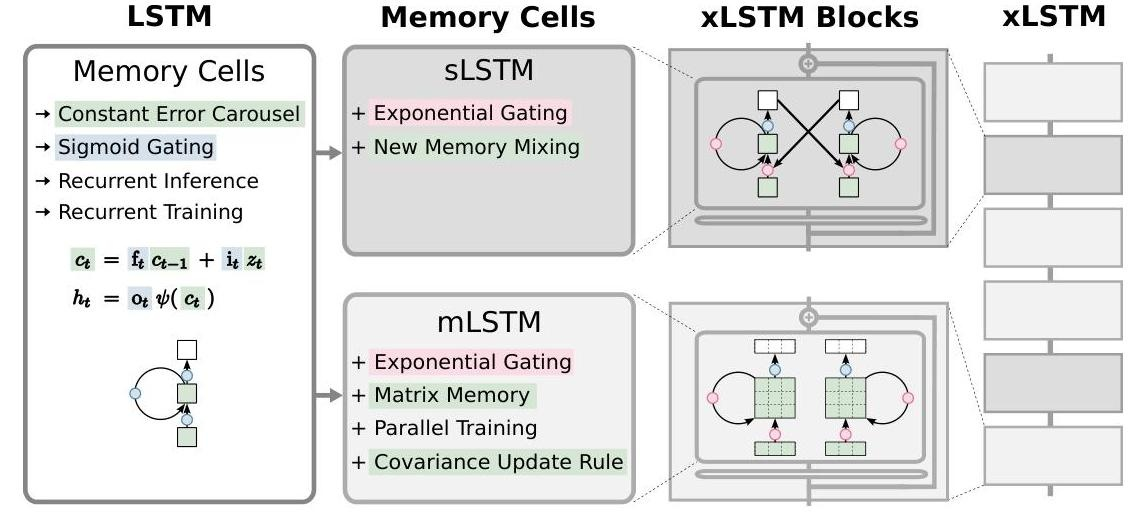
\includegraphics[width=0.95\linewidth]{images/xlstm_extracted_images/page_1_img-0.jpeg}
\caption{
    xLSTM architecture components (adapted from~\cite{beck2024xlstm}). The progression shows: (1) traditional LSTM structure with its constant error carousel mechanism, (2) two proposed cell variants (sLSTM and mLSTM) that employ exponential gate activations, (3) block-level integration with residual pathways, (4) full architecture formed by stacking multiple blocks.
}\label{fig:xlstm_overview}
\end{figure}

\subsection{Limitations of Traditional LSTMs}

The xLSTM work~\cite{beck2024xlstm} identifies several architectural constraints in traditional \acp{LSTM}~\cite{hochreiter1997lstm} that motivated the design:

\begin{figure}[t]
\centering
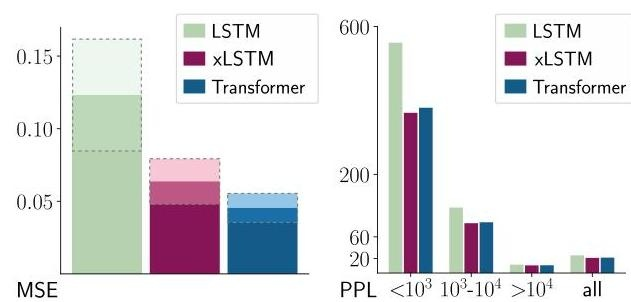
\includegraphics[width=0.95\linewidth]{images/xlstm_extracted_images/page_2_img-1.jpeg}
\caption{
    Empirical demonstration of LSTM architectural constraints (adapted from~\cite{beck2024xlstm}). Two synthetic tasks highlight different issues: the Nearest Neighbor Search task (left panel, measured by MSE) reveals difficulties in updating stored information when new relevant data arrives, while the Rare Token Prediction task (right panel, measured by perplexity) shows degradation in performance for infrequent patterns.
}\label{fig:lstm_limitations}
\end{figure}

\begin{enumerate}
    \item \textbf{Fixed Memory Commitment}: The scalar cell state architecture makes it difficult to overwrite previously stored information when more relevant data becomes available later in the sequence.
    
    \item \textbf{Scalar Memory Bottleneck}: Compressing information into single scalar values per cell constrains the model's capacity to represent multiple concurrent patterns or features.
    
    \item \textbf{Inherent Sequential Dependency}: The recurrent formulation requires processing steps in strict temporal order, which prevents parallel computation during training and limits throughput compared to architectures like Transformers.
\end{enumerate}

\subsection{xLSTM Innovations}

The xLSTM architecture~\cite{beck2024xlstm} introduces two main modifications to the traditional LSTM structure: a different gate activation scheme and redesigned memory representations.

\subsubsection{Exponential Gating}

The standard \ac{LSTM} employs sigmoid functions for gate activations, which compress values to the $(0,1)$ range. The xLSTM design replaces these with exponential activations:

$$\tilde{f}_t = \exp(f_t), \quad \tilde{i}_t = \exp(i_t)$$

where $f_t$ and $i_t$ denote pre-activation values for the forget and input gates. The exponential function provides a wider effective dynamic range and modifies gradient propagation behavior, which may facilitate improved learning dynamics~\cite{beck2024xlstm}.

\textbf{Numerical Stabilization:} Since exponentials can grow unbounded, a stabilization mechanism is introduced~\cite{beck2024xlstm}. An auxiliary variable $m_t$ maintains the logarithmic maximum:

\begin{align}
m_t &= \max(\log(f_t) + m_{t-1}, \log(i_t)) \\
i_t' &= \exp(\log(i_t) - m_t) = \exp(\tilde{i}_t - m_t) \\
f_t' &= \exp(\log(f_t) + m_{t-1} - m_t)
\end{align}

The stabilized gates $f_t'$ and $i_t'$ are then used in the forward pass, ensuring numerical stability without changing the model's outputs or gradients.

\subsubsection{Memory Structure Innovations}

\ac{xLSTM} introduces two distinct memory architectures:

\paragraph{Scalar LSTM (sLSTM)}
The \ac{sLSTM} variant maintains scalar-valued memory cells, similar to traditional \acp{LSTM}, but incorporates the exponential gate activations described above. The cell state evolution follows:

\begin{align}
c_t &= \tilde{f}_t \odot c_{t-1} + \tilde{i}_t \odot z_t \\
n_t &= \tilde{f}_t \odot n_{t-1} + \tilde{i}_t \\
h_t &= o_t \odot \frac{c_t}{n_t}
\end{align}

where $\tilde{f}_t = \exp(f_t)$ and $\tilde{i}_t = \exp(i_t)$ denote the exponential gate values, while $z_t$ represents the input content. The additional variable $n_t$ accumulates gate contributions to normalize the output. This formulation allows the forget gate to more aggressively remove outdated information when $\tilde{f}_t$ is small.

\paragraph{Matrix LSTM (mLSTM)}
The \ac{mLSTM} variant uses matrix-valued memory $\mathbf{C}_t \in \mathbb{R}^{d \times d}$ instead of scalar cells. This design~\cite{beck2024xlstm} provides several properties:

\begin{itemize}
    \item \textbf{Increased Information Capacity}: Matrix storage allows representing multiple patterns simultaneously through structured key-value interactions.
    
    \item \textbf{Parallel Training}: The architecture removes recurrence between hidden states, enabling parallelization across the sequence dimension during training.
    
    \item \textbf{Associative Updates}: Memory updates use outer products between vectors, creating rank-one modifications to the memory matrix.
\end{itemize}

The memory dynamics are defined as:

\begin{align}
\mathbf{C}_t &= f_t \odot \mathbf{C}_{t-1} + i_t \odot \mathbf{v}_t \mathbf{k}_t^{\top} \\
\mathbf{n}_t &= f_t \odot \mathbf{n}_{t-1} + i_t \odot \mathbf{k}_t \\
\mathbf{h}_t &= \mathbf{o}_t \odot \frac{\mathbf{C}_t \mathbf{q}_t}{\max\{|\mathbf{n}_t^{\top} \mathbf{q}_t|, 1\}}
\end{align}

Here $f_t$, $i_t$, $\mathbf{o}_t$ are gate values (with exponential activations), while $\mathbf{v}_t$, $\mathbf{k}_t$, $\mathbf{q}_t$ are the value, key, and query projections of the input. The normalizer $\mathbf{n}_t$ accumulates key vectors to stabilize the retrieval operation in the third equation.

\subsection{xLSTM Block Architecture}

\ac{xLSTM} components are integrated into residual block architectures, similar to Transformer blocks. Each \ac{xLSTM} block contains:

\begin{itemize}
    \item Layer normalization for stable training
    \item Residual connections for gradient flow
    \item Feed-forward networks for non-linear transformations
    \item Dropout for regularization
\end{itemize}

Multiple \ac{xLSTM} blocks can be stacked to create deep architectures that combine the benefits of both \ac{sLSTM} and \ac{mLSTM} components.

\subsection{Potential Relevance for Biosignal Processing}

The xLSTM modifications~\cite{beck2024xlstm} may offer certain properties relevant to biosignal analysis:

\begin{itemize}
    \item \textbf{Temporal Dependency Modeling}: Exponential gate activations provide a different mechanism for weighting temporal relationships, which could be relevant for biosignals where event timing carries clinical significance.
    
    \item \textbf{Dynamic Memory Allocation}: The modified gating scheme allows the network to adjust what information is retained as the sequence progresses, potentially useful when processing long recordings where later segments may contradict earlier ones.
    
    \item \textbf{Training Efficiency}: The \ac{mLSTM} variant enables parallel computation during training by removing hidden-to-hidden recurrence, while \ac{sLSTM} maintains sequential dependencies but can leverage optimized implementations.
    
    \item \textbf{Representational Capacity}: Matrix-valued memory in \ac{mLSTM} provides higher-dimensional storage that could model complex relationships in multi-channel data through its associative update mechanism.
    
    \item \textbf{Sequential State Maintenance}: The \ac{sLSTM} variant with its recurrent structure may handle tasks requiring explicit state tracking across time, which could be relevant for monitoring evolving biosignal patterns.
\end{itemize}


\section{Integration of xLSTM with BIOT}
\label{sec:background:integration}

Integrating \ac{xLSTM} architectures into the \ac{BIOT} framework is a natural next step that combines the strengths of both approaches. This section describes the theoretical foundation for this integration and its potential benefits.

\subsection{Architectural Compatibility}

\ac{BIOT}'s modular design enables straightforward integration of \ac{xLSTM} components as alternatives to the Linear Transformer encoder. The integration maintains the complete biosignal tokenization pipeline:

\begin{enumerate}
    \item \textbf{Tokenization Module}: The resampling, normalization, \ac{STFT}-based segmentation, and embedding components remain unchanged, preserving \ac{BIOT}'s ability to handle heterogeneous biosignal formats.
    
    \item \textbf{Sequence Processing}: The Linear Transformer blocks are replaced with \ac{xLSTM} block stacks (\ac{sLSTM}, \ac{mLSTM}, or hybrid combinations), enabling evaluation of different memory mechanisms.
    
    \item \textbf{Aggregation}: Sequence representations are aggregated via mean pooling across tokens before classification, consistent with the original \ac{BIOT} approach.
\end{enumerate}

This modular replacement allows systematic comparison of sequence modeling approaches while preserving the key advantages of \ac{BIOT}'s flexible tokenization strategy.

\subsection{Theoretical Synergies}

Combining \ac{BIOT} tokenization with \ac{xLSTM} processing offers several theoretical advantages:

\begin{itemize}
    \item \textbf{Preserved Flexibility}: \ac{BIOT}'s tokenization approach keeps compatibility with different biosignal formats while \ac{xLSTM} provides enhanced sequence processing.
    
    \item \textbf{Enhanced Temporal Modeling}: \ac{xLSTM}'s superior memory mechanisms could better capture the complex temporal patterns in biosignals.
    
    \item \textbf{Scalable Performance}: The combination maintains computational efficiency while potentially improving classification accuracy.
    
    \item \textbf{Cross-dataset Applicability}: The integration preserves \ac{BIOT}'s ability to work across different datasets while potentially improving performance through better sequence modeling.
\end{itemize}

\subsection{Expected Benefits}

From a theoretical perspective, integrating \ac{xLSTM} with \ac{BIOT} could address several limitations:

\begin{itemize}
    \item \textbf{Improved Long-range Dependencies}: \ac{xLSTM}'s enhanced memory capabilities could better capture dependencies across long biosignal sequences.
    
    \item \textbf{Better Pattern Recognition}: The matrix memory structures in \ac{mLSTM} could enable more sophisticated pattern recognition in multi-channel biosignals.
    
    \item \textbf{Enhanced Robustness}: \ac{xLSTM}'s ability to revise storage decisions could improve robustness to noise and artifacts that are common in biosignals.
\end{itemize}

This theoretical foundation is why this thesis evaluates \ac{xLSTM} variants within the \ac{BIOT} framework, which is the focus of the following experimental chapters.


%% 
%%%%%%%%%%%%%%%%%%%%%%%%%%%%%%%%%%%%%%%%%%%%%%%%%%%%%%%%%%%%%%%%%%%%%%%%%%%%%%%%
